

\documentclass[12pt,a4paper]{article}
\newcommand\persiangloss[2]{#1\dotfill\lr{#2}\\}
\usepackage{graphicx}
\usepackage{xcolor}
\usepackage{listings}
\usepackage{indentfirst}
\usepackage{float}
\usepackage[pagebackref=false,colorlinks,linkcolor=blue,citecolor=magenta]{hyperref}
\usepackage{xepersian}
\settextfont{XB Niloofar}
\definecolor{vgreen}{RGB}{104,180,104}
\definecolor{vblue}{RGB}{49,49,255}
\definecolor{vorange}{RGB}{255,143,102}

\lstdefinestyle{verilog-style}
{
	language=Verilog,
	basicstyle=\small\ttfamily,
	keywordstyle=\color{vblue},
	identifierstyle=\color{black},
	commentstyle=\color{vgreen},
	numbers=left,
	numberstyle=\tiny\color{black},
	numbersep=10pt,
	tabsize=8,
	moredelim=*[s][\colorIndex]{[}{]},
	literate=*{:}{:}1
} 


\defpersianfont\traffic[Scale=1]{B Roya}
\defpersianfont\yekan[Scale=1]{XB Kayhan}

\begin{document}
	\thispagestyle{empty}
	\vspace*{0mm}
	\centerline{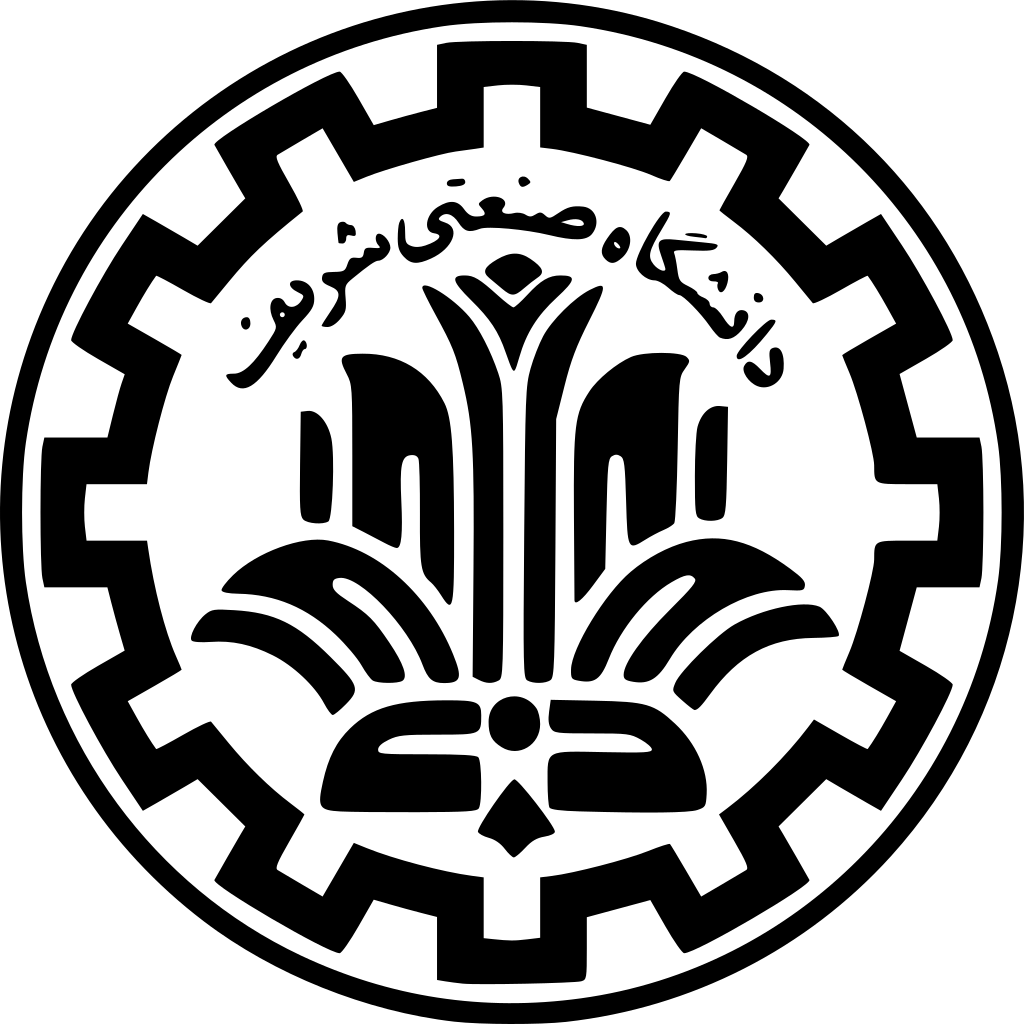
\includegraphics[height=4cm]{logo.png}}
	\vspace*{5mm}
	\begin{center}
		{\yekan \Huge
لوستر هوشمند - گزارش اول
}
\\[1cm]
آزمایشگاه سخت‌افزار
\\[1cm]
دانشکده مهندسی کامپیوتر
\\[4cm]
{\large \traffic
محمدرضا عبدی ۹۷۱۱۰۲۸۵

حمیدرضا کامکاری ۹۷۱۱۰۱۷۷

یگانه قره‌داغی 97106216
}
	\\[5cm]
	فروردین ۱۴۰۱
	\end{center}
\newpage

\section*{گزارش مرحله اول}

در این آزمایش با روند کلی بستن آردویینو و برنامه‌نویسی اولیه‌ آن آشنا شدیم و تلاش کردیم تعدادی \lr{LED} را به صورت شبکه‌ای بسته و شدت نور آن را تنظیم کنیم. هدف کلی بستن ۶۰ تا چراغ \lr{LED} بود اما در این گزارش به دلیل اینکه هدف آشنایی بود صرفا ۶ تا \lr{LED} را به صورت موازی و به پین‌های مختلف وصل کرده و تنظیم کردیم. نهایتاً برنامه‌ای نوشتیم که به ترتیب \lr{LED} ها را به صورت تدریجی از کمترین شدت به بیشترین شدت و سپس برعکس روشن می‌کند و در نهایت این مراحل را از ابتدا انجام می‌دهد.

در ابتدای کار پکیج \lr{Arduino Mega} داده شده را بستیم و \lr{driver} مربوطه به همراه ویرایشگر مرتبطش را راه‌اندازی کردیم. سپس بردبورد را مشابه تصویر زیر بستیم به طوری‌که ۶ تا \lr{LED} به پین‌های \lr{digital PWM} از شماره 2 تا 7 متصل شدند. همچنین برای جلوگیری از احتمال سوختن \lr{LED} از مقاومت‌های $ 1k \Omega$ استفاده کردیم.
\begin{figure}[H]
	\centering
	\includegraphics[scale=0.085]{figs/all.png}
	\caption{روشن شدن تمامی \lr{LED} ها}
	\label{fig4}
\end{figure}

هدف اولیه‌مان این بود که شبکه را با استفاده از ۶۰ تا \lr{LED} دریافت شده به صورت کامل ببندیم اما هنگامی که ۳ تا \lr{LED} را به صورت متوالی بستیم مشاهده کردیم که مقدار ولتاژ خروجی از بورد \lr{Arduino} کفاف نمی‌دهد. لذا به ازای هر رشته متوالی از لوستر باید از یک آمپلیفایر یا منبع تغذیه خارجی مثل یک باتری به کمک یک مقاومت متغیر برای تنظیم نور بهره‌بگیریم. در هر حال، صرفا برای تست کردن ابزار آلات هر رشته را فعلا تک LED در نظر گرفتیم و کد‌های مربوطه را روی آن امتحان کردیم.

همانطور که در کد زیر دیده می‌شود، برنامه اولیه‌مان به ترتیب شدت نور ۶ تا \lr{LED} از لوستر را تنظیم می‌کند. با استفاده از پین‌های \lr{PWM} می‌توانیم به صورت دیجیتال شدت نور خروجی را عددی بین 0 تا 255تنظیم کنیم و این کاری است که در کد کرده‌ایم. برای دیدن نتیجه، ویدیویی به این گزارش پیوست شده که خروجی این کد را روی بورد نشان می‌دهد.
\begin{latin}
	\lstinputlisting[style={verilog-style}]{src/Serial.ino}
\end{latin}

\end{document}